\documentclass[border=3pt,tikz]{standalone}
\usepackage{amsmath}
\usetikzlibrary{calc}
\usetikzlibrary{arrows.meta} % for arrow size
\usetikzlibrary{calc}
\begin{document}
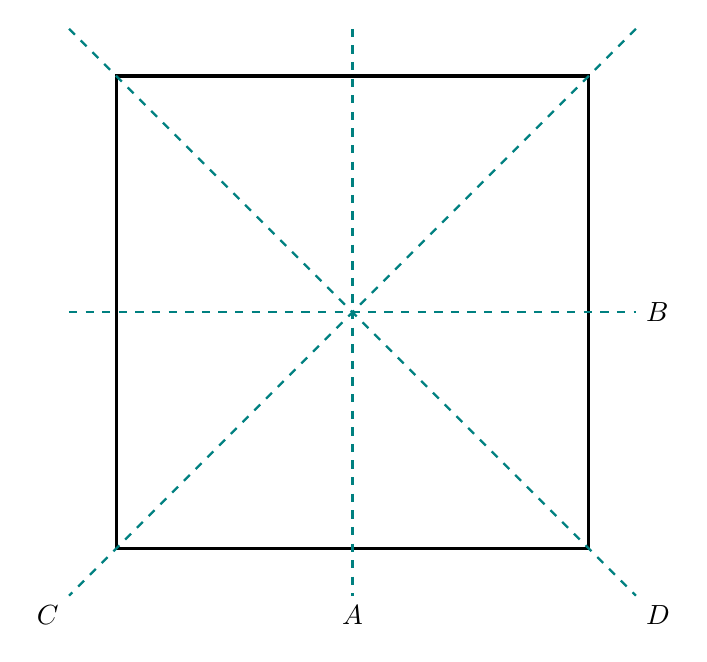
\begin{tikzpicture}[scale=3, extended line/.style={shorten >=-#1,shorten <=-#1},
    extended line/.default=1cm]
    
    \coordinate (P1) at (1, -1);
    \coordinate (P2) at (1,1);
    \coordinate (P3) at (-1,1);
    \coordinate (P4) at (-1,-1);
    
    
    
    \draw[very thick] (P1) -- (P2) -- (P3) -- (P4) -- cycle;

    \draw[thick, teal, dashed] (1.2, 1.2) -- (-1.2, -1.2) node [below left, black] {$C$};
    \draw[thick, teal, dashed] (-1.2, 1.2) -- (1.2, -1.2) node [below right, black] {$D$};
    \draw[thick, teal, dashed] (0, 1.2) -- (0, -1.2) node [below, black] {$A$};
    \draw[thick, teal, dashed] (-1.2, 0) -- (1.2, 0) node [right, black] {$B$};
    

    \end{tikzpicture}
\end{document}